\chapter{Overall Description}
\label{chap:overall_description}%

\section{Product Perspective}
\label{sec:product_perspective}%

\subsection{Scenarios}
\label{sub:scenarios}%

\par{\textbf{Scenario 1: Registered User Creates an Account and Records a Trip}}
Emma R.\ is a regular cyclist who wants to keep track of her personal bike activity. She installs the Best Bike Paths (BBP) mobile application and creates an account by providing basic identification and contact information. Once her account is verified, she can access the app’s personalised features.

During her daily commute, Emma decides to record her ride. She starts a new trip and BBP automatically collects GPS data, speed, and performance-related statistics. At the end of the route, the system stops the recording and stores the trip in her private dashboard. BBP also retrieves contextual meteorological information (temperature, weather conditions) for that time interval from an external service. Emma can later review her rides and aggregated statistics through her personal area.

\par{\textbf{Scenario 2: Manual Definition and Publication of a Bike Path}}
Luca P.\ is an experienced cyclist who wants to publish a safe route that is not well documented in existing map services. He accesses BBP with his registered account and uses the manual path creation feature to define a custom bike route.

BBP provides map-based tools and a street search mechanism that allow Luca to select the relevant street segments and assign each segment a status (such as optimal, medium, or requiring maintenance). He may also optionally indicate obstacles identified along the route. Once satisfied with the defined path, he assigns it a name and publishes it. The system computes a score for the new route based on the provided data, making it available to all users performing searches in that area.

\par{\textbf{Scenario 3: Automatic Trip Recording with Sensor-Based Obstacle Detection}}
Sara C.\ wants to contribute information about the conditions of a road she frequently uses. She activates BBP’s automatic trip recording, which uses GPS data together with available mobile sensors (such as accelerometer and gyroscope) to detect potential anomalies along the route. 

During her ride, the system identifies unusual vibrations or irregularities that might correspond to obstacles. After the trip ends, BBP presents Sara with a summary of the detected points and asks her to confirm or correct the interpretation of the obstacles, ensuring false positives are handled. Once validated, the information is stored and may enrich the quality of future published paths and their scores.

\par{\textbf{Scenario 4: Casual User Searches for a Path Between Two Locations}}
Marco L.\ is visiting a city for a weekend and wants to reach a park starting from his hotel using a safe bike route. Without creating an account, he accesses BBP as a casual user and specifies his starting point and destination.

BBP identifies the available routes matching the query and ranks them according to their score, which reflects factors such as route condition and overall status.  Marco inspects the proposed alternatives and visualises the most suitable route on the map. Even without registering, he can use BBP to safely reach his destination.

\par{\textbf{Scenario 5: Registered User Publishes and Later Updates a Frequently Used Path}}
After several weeks of using BBP, Emma R.\ notices that her recurring commuting route is not available as a public path. She selects one of her recorded private trips and uses BBP’s functionality to derive a candidate publishable path. She verifies the correctness of the route and adjusts the status of certain segments based on her experience. After assigning a name to the path, she publishes it, making it available to other users.

\par{\textbf{Scenario 6: User Updates an Existing Path with New Data}}
Tom H.\ has recently moved to the city and uses BBP to find a reliable bike route between his home and the train station. While following the suggested route, he starts recording his trip through the application. Once the ride is completed, he reviews the automatically detected information and assigns the road status as optimal. In the BBP database, that same path was previously rated as medium by other users. Since Tom provides publishable information, BBP updates the stored data by incorporating his contribution. The system re-evaluates the score of the path by considering the freshness of Tom's input and the number of previous submissions. If Tom's assessment is consistent with other recent reports, the aggregated status is adjusted accordingly; otherwise, the system keeps the data until further contributions resolve the conflict.

\subsection{Class Diagram}
\label{sub:class_diagram}

\begin{figure}[H]
    \centering
    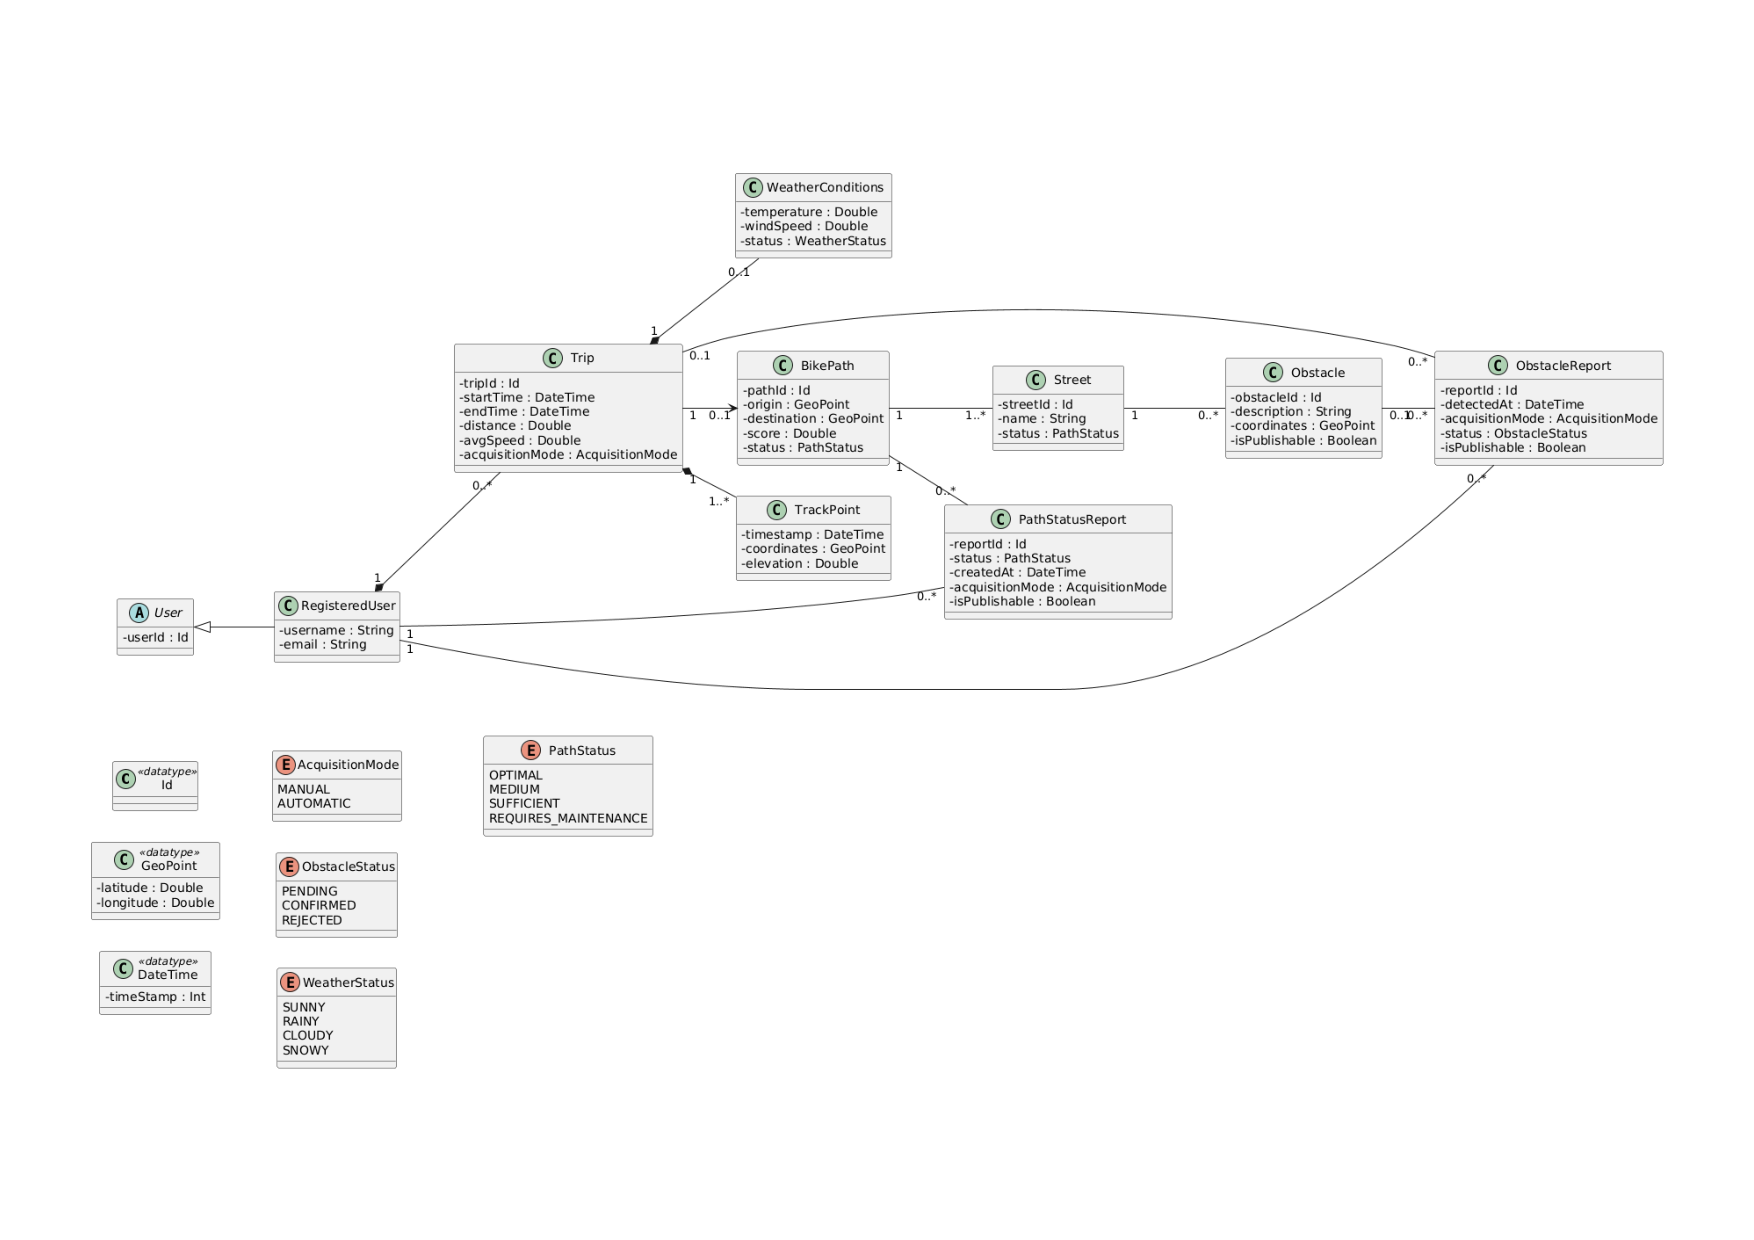
\includegraphics[width=1.0\textwidth]{Images/UML/UML.pdf}
    \caption{High Level View - Class Diagram}
    \label{fig:class_diagram}
\end{figure}

\par The class diagram in Figure~\ref{fig:class_diagram} presents the conceptual domain model of the \textit{Best Bike Paths} system. It focuses on the main entities and relationships that characterize cycling activities, reported obstacles, path conditions, and contextual information. This diagram does not describe how the system is implemented. Architectural aspects, technical components, and service interfaces for data acquisition and processing will be introduced and detailed later in the Design Document (DD).

\par At the core of the model is the abstraction \texttt{User}, specialized by \texttt{RegisteredUser}. A \texttt{RegisteredUser} represents an authenticated user of the platform, identified by a unique \texttt{userId} and characterized by basic account information such as \texttt{username} and \texttt{email}. Each registered user can own multiple \texttt{Trip} instances, corresponding to the cycling activities recorded over time.

\par A \texttt{Trip} describes a single cycling session. It stores a unique \texttt{tripId}, the \texttt{startTime} and \texttt{endTime}, the total \texttt{distance}, the \texttt{avgSpeed}, and an \texttt{acquisitionMode} attribute indicating whether the trip was collected manually or automatically. A trip is decomposed into a sequence of \texttt{TrackPoint} objects, related to the trip through a composition. Each \texttt{TrackPoint} carries a \texttt{timestamp}, a geographic position (\texttt{coordinates} of type \texttt{GeoPoint}), and an \texttt{elevation}, capturing the detailed trace followed by the cyclist.

\par Trips can optionally be associated with a \texttt{BikePath}, which represents a meaningful route between two \texttt{GeoPoint} locations (\texttt{origin} and \texttt{destination}). A \texttt{BikePath} maintains an overall \texttt{score} and a \texttt{status} of type \texttt{PathStatus}, reflecting its current quality (for example optimal, medium, sufficient, or requiring maintenance). Each bike path is composed of one or more \texttt{Street} objects. A \texttt{Street} is identified by a \texttt{streetId} and a \texttt{name}, and it also holds a \texttt{status} of type \texttt{PathStatus} to represent the condition of that specific segment of the path.

\par The model explicitly represents user feedback on path quality through the \texttt{PathStatusReport} class. A \texttt{PathStatusReport} describes a single contribution provided by a user about the condition of a given \texttt{BikePath}. It includes a unique \texttt{reportId}, the reported \texttt{status} (\texttt{PathStatus}), the \texttt{createdAt} timestamp, and the \texttt{acquisitionMode} that distinguishes between manually entered and automatically derived feedback. The \texttt{isPublishable} flag indicates whether this piece of information can be made available to other users. Each \texttt{PathStatusReport} is associated with exactly one \texttt{RegisteredUser} and one \texttt{BikePath}, and the collection of reports contributes to the aggregated score and status maintained by the path.

\par Obstacles along the streets are modeled through the \texttt{Obstacle} and \texttt{ObstacleReport} classes. An \texttt{Obstacle} represents a consolidated unsafe element on the infrastructure, such as a pothole or an irregular surface. It has a unique \texttt{obstacleId}, a textual \texttt{description}, a position given by \texttt{coordinates}, and an \texttt{isPublishable} attribute specifying whether the obstacle is visible to the community. Obstacles are linked to \texttt{Street} objects, indicating on which street they are located. The life cycle and validation of obstacles are represented by \texttt{ObstacleReport}. Each \texttt{ObstacleReport} records a detection event with a unique \texttt{reportId}, the \texttt{detectedAt} time, the \texttt{acquisitionMode} (manual or automatic), and a \texttt{status} of type \texttt{ObstacleStatus}, which can be pending, confirmed, or rejected. The \texttt{isPublishable} attribute mirrors whether that specific report can be shared. Reports are created by \texttt{RegisteredUser} instances, may originate during a \texttt{Trip}, and can optionally be associated with a consolidated \texttt{Obstacle}. This allows the system to represent both preliminary detections and validated obstacles confirmed by multiple users.

\par Environmental context for each trip is captured by the \texttt{WeatherConditions} value object. A \texttt{Trip} may own at most one \texttt{WeatherConditions} instance, modeled as a composition. This class stores temperature, wind speed, and a \texttt{status} of type \texttt{WeatherStatus} (such as sunny, rainy, cloudy, or snowy), thus enriching the activity with information about the weather at the time it was performed.

\par The diagram also includes simple data types and enumerations used across the domain. Identifiers are abstracted as \texttt{Id}, spatial positions as \texttt{GeoPoint}, and timestamps as \texttt{DateTime}. The \texttt{AcquisitionMode} enumeration distinguishes manual and automatic data acquisition. \texttt{PathStatus}, \texttt{ObstacleStatus}, and \texttt{WeatherStatus} enumerate the possible qualitative states for paths, obstacles, and weather respectively.

\par Overall, this class diagram describes the problem domain relevant to \textit{Best Bike Paths}. It shows how user activities, routes, streets, obstacles, feedback on path quality, and contextual weather conditions are structured and interrelated at a conceptual level. It does not prescribe how these entities are stored, accessed, or computed at runtime. Such architectural and implementation details, including components for sensor management, trip recording, external map or weather services, and their interfaces, are intentionally omitted from the RASD domain model and will be addressed in the Design Document.

\subsubsection{Clarifications on Domain Modeling Consistency}
\label{sub:domain_modeling_clarifications}

\par The class diagram in Figure~\ref{fig:class_diagram} adopts a conceptual modeling approach that intentionally abstracts from implementation and persistence details. Some design choices are clarified below to ensure full consistency between the textual description and the UML model.

\par Trips are modeled as being owned by a \texttt{RegisteredUser} through a composition relationship. This implies a strong lifecycle dependency: a \texttt{Trip} cannot exist independently of its owning user and is removed if the corresponding account is deleted. While this dependency is not always made explicit in the scenarios, it is assumed throughout the domain model.

\par The notion of publication for trips and bike paths is treated as a process-level concern rather than a structural property of the domain entities. Consequently, the \texttt{BikePath} class does not include explicit attributes such as \texttt{isPublishable} or \texttt{publishedAt}. A bike path is considered publicly available when it exists in the shared dataset and is supported by publishable user contributions, such as validated \texttt{PathStatusReport} instances. The rules governing visibility and publication are enforced by application logic and are therefore intentionally excluded from the domain model.

\par Environmental information is modeled at the level of individual trips through the \texttt{WeatherConditions} value object, which is optionally composed by a \texttt{Trip}. This reflects the assumption that meteorological data is contextual to the time and location of a specific cycling activity and is not aggregated or shared across multiple trips or bike paths.

\par Although the system allows both registered and unregistered cyclists to interact with the application, only registered users are represented as persistent entities in the domain model. Unregistered cyclists are treated as transient actors who can access and visualize aggregated information without being explicitly modeled as domain objects.

\par These clarifications ensure that the textual description, scenarios, and functional requirements remain fully aligned with the conceptual structure expressed by the UML class diagram, while preserving a clear separation between domain modeling and architectural or implementation concerns.

\section{Product Functions}
\label{sec:product_functions}%

\par The following section describes the main functions of the system.
\begin{itemize}

  \item \textbf{Account creation}:

The account creation process allows a visitor to register as a BBP user through a structured and controlled workflow involving both user-side interactions and backend validations. The process starts when the visitor opens the sign-in page and submits a proposed email address. The BBP backend first checks whether the email is already associated with an existing account. If the user is already registered, the process is aborted and an appropriate notice is issued.

If the email is not registered, the user is asked to insert and confirm a password. This step is governed by a subprocess that verifies compliance with security requirements and checks that the two password entries correspond. In case of non-compliance or mismatch, error messages are returned and the user is allowed to retry, with the number of attempts being monitored. If the maximum number of attempts is exceeded, the process is aborted.

Once valid credentials are provided, the backend registers the user in a provisional state and sends a confirmation email containing a verification code. The user must then insert the received confirmation code within a defined time window. This verification phase includes multiple subprocesses handling incorrect codes, timeouts, and email resend requests. The system limits both the number of code insertion attempts and the number of resend requests. Exceeding these limits results in a timeout or process termination with an explicit notice.

If the confirmation code is correct and received within the allowed constraints, the registration is finalized and the user account is activated. Upon successful confirmation, the user can immediately start editing their profile. The completion of this process grants access to all core BBP functionalities, including recording and storing personal cycling trips, viewing statistics, and actively contributing to the platform by publishing information on bike path conditions and obstacles.

            \begin{figure}[H]
                  \centering
                  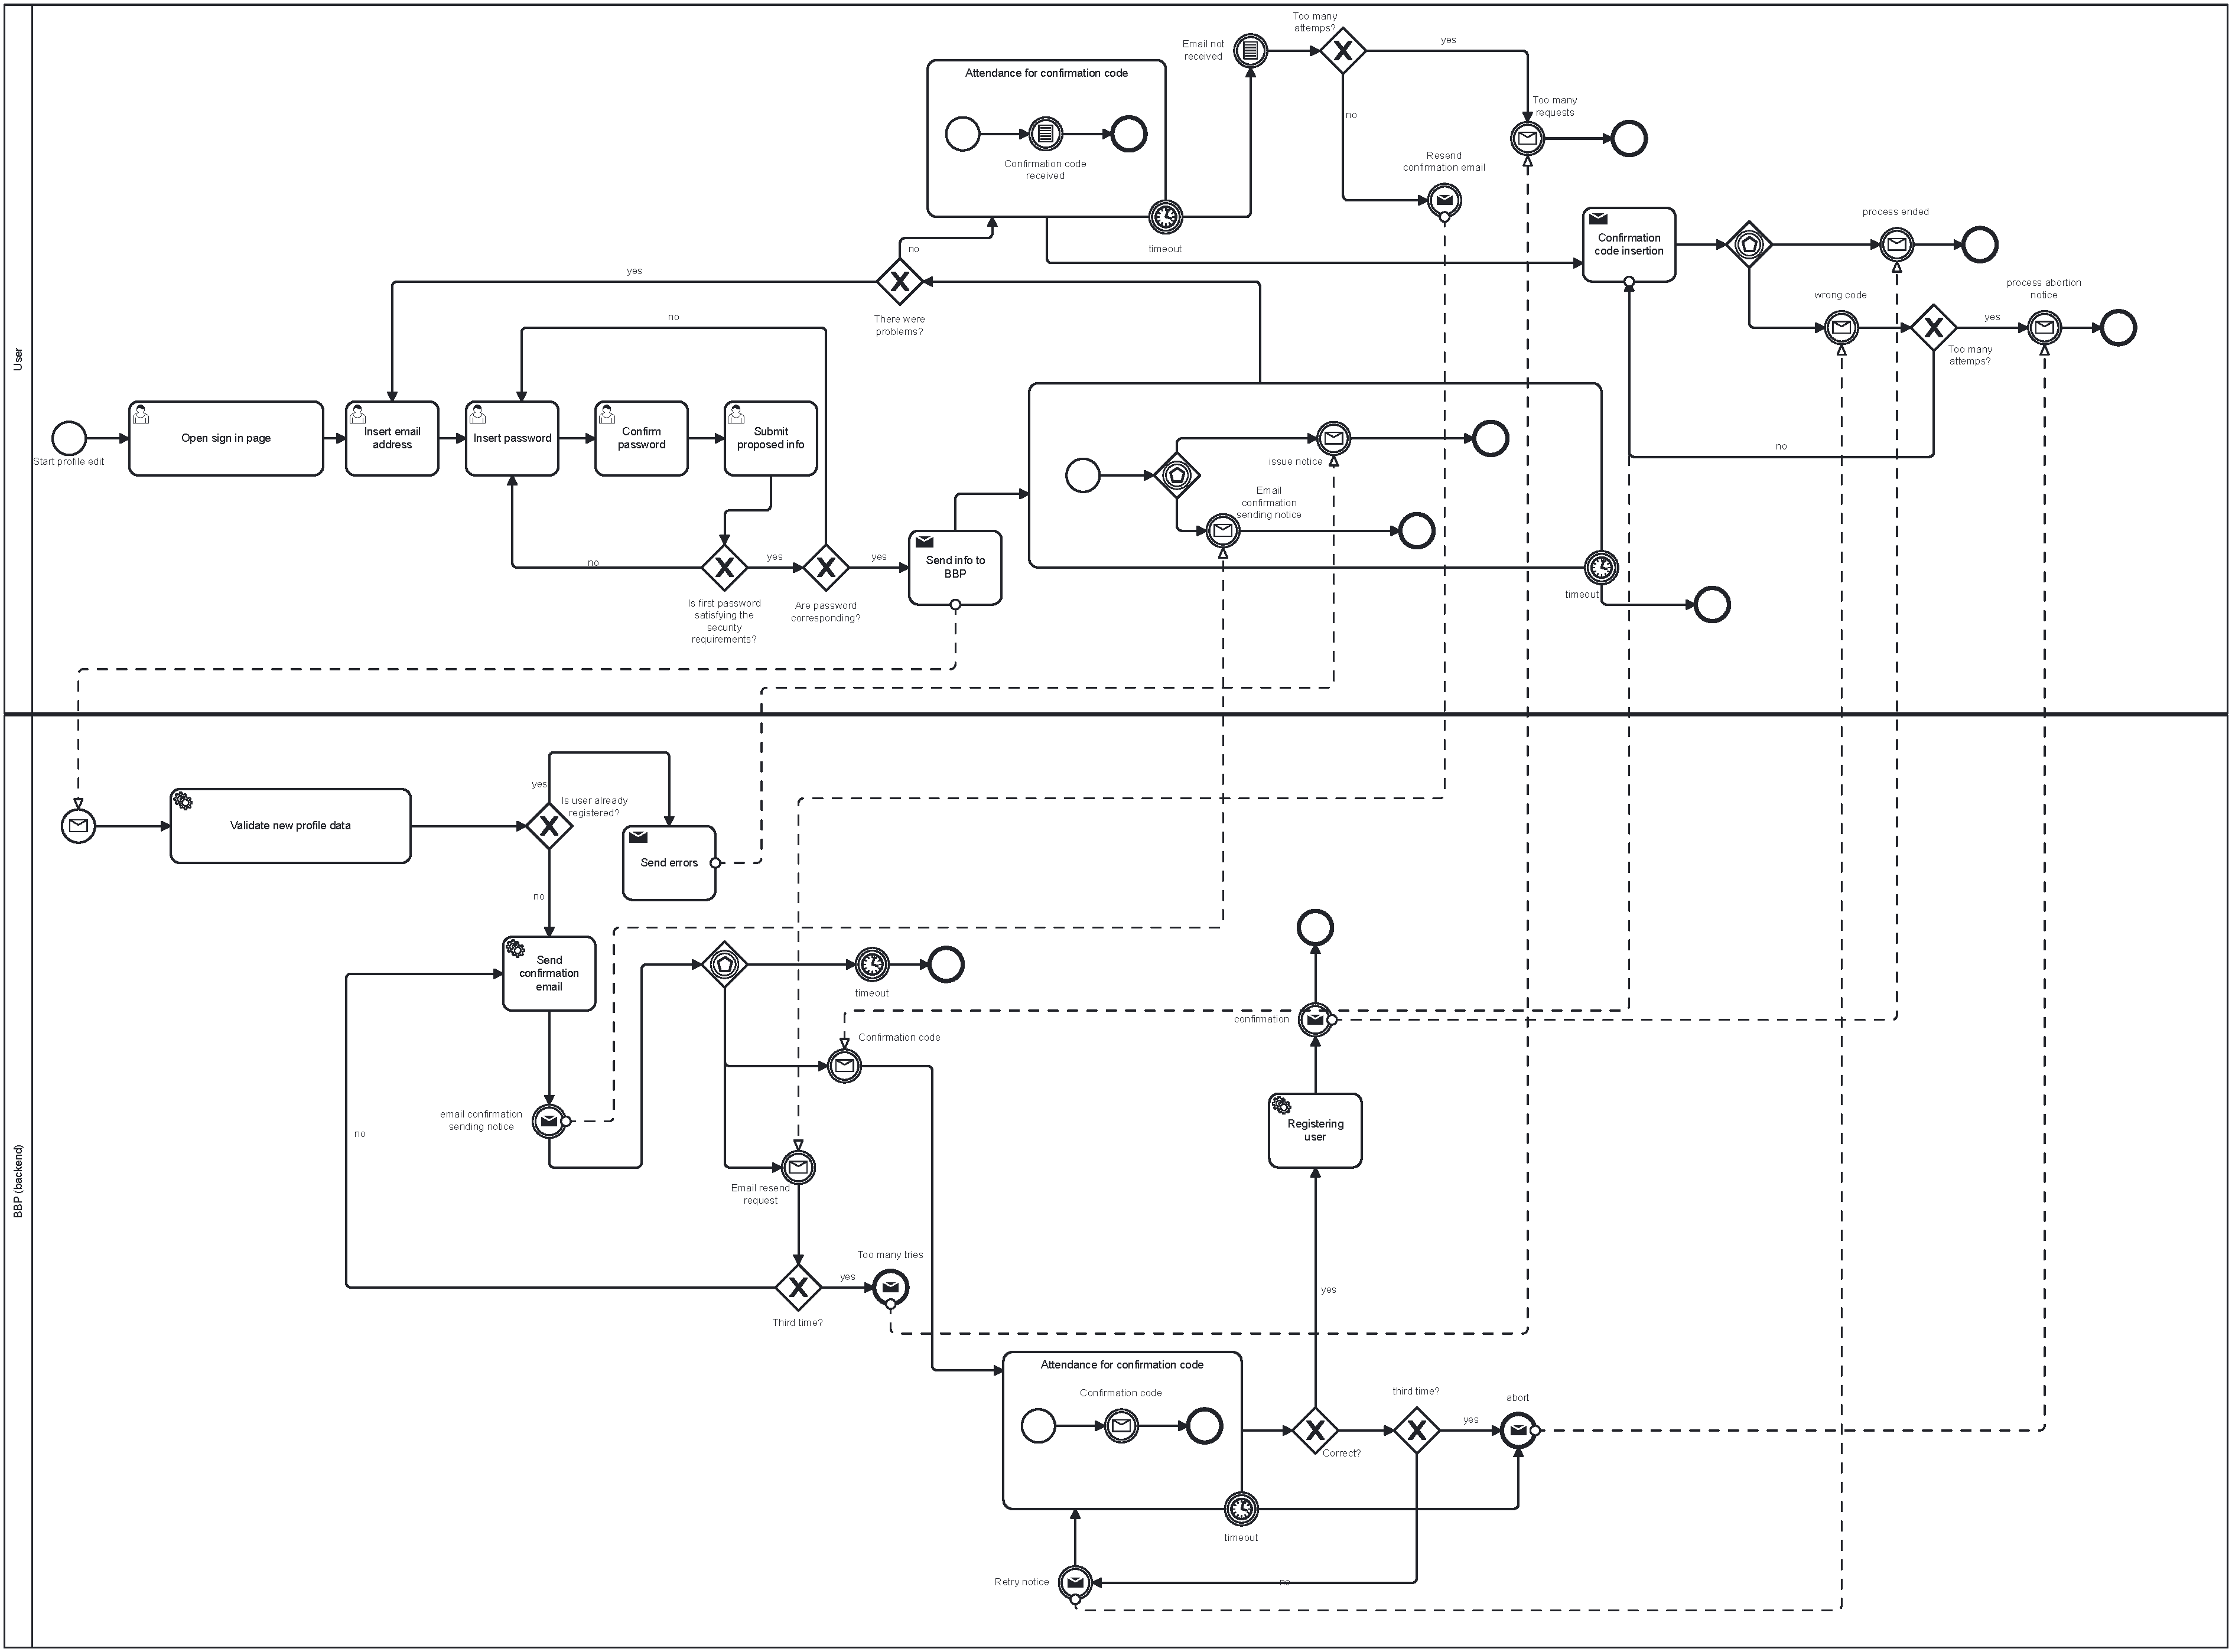
\includegraphics[width=1.0\textwidth]{Images/BPMN/create-an-account.pdf}
                  \caption{Account Creation - Product Function}
                  \label{fig:create-an-account}
            \end{figure}
\end{itemize}


\begin{itemize}
      \item \textbf{Edit Profile}:

The Edit Profile functionality enables authenticated users to update and maintain their personal information within the Best Bike Paths system through a controlled interaction with the backend services. The process starts when the user accesses their profile page and explicitly opens the edit mode. At this stage, the system exposes editable profile fields, excluding the email address, which is managed through a separate confirmation-driven process.

The user can modify personal attributes such as display preferences or other non-sensitive identification data. Once the changes are submitted, the BBP backend executes a validation subprocess to verify data consistency, format correctness, and compliance with system constraints. If validation errors are detected, the system returns detailed feedback, allowing the user to correct the input and resubmit the data.

If the provided information is valid, the backend updates the user profile in the database and sends a confirmation notice to the user, signaling the successful completion of the operation. The process also accounts for exceptional situations, such as inactivity timeouts, in which case the edit session is terminated and an explicit notice is issued. Upon successful update, all subsequent interactions with the platform reflect the newly stored profile information.

            \begin{figure}[H]
                  \centering
                  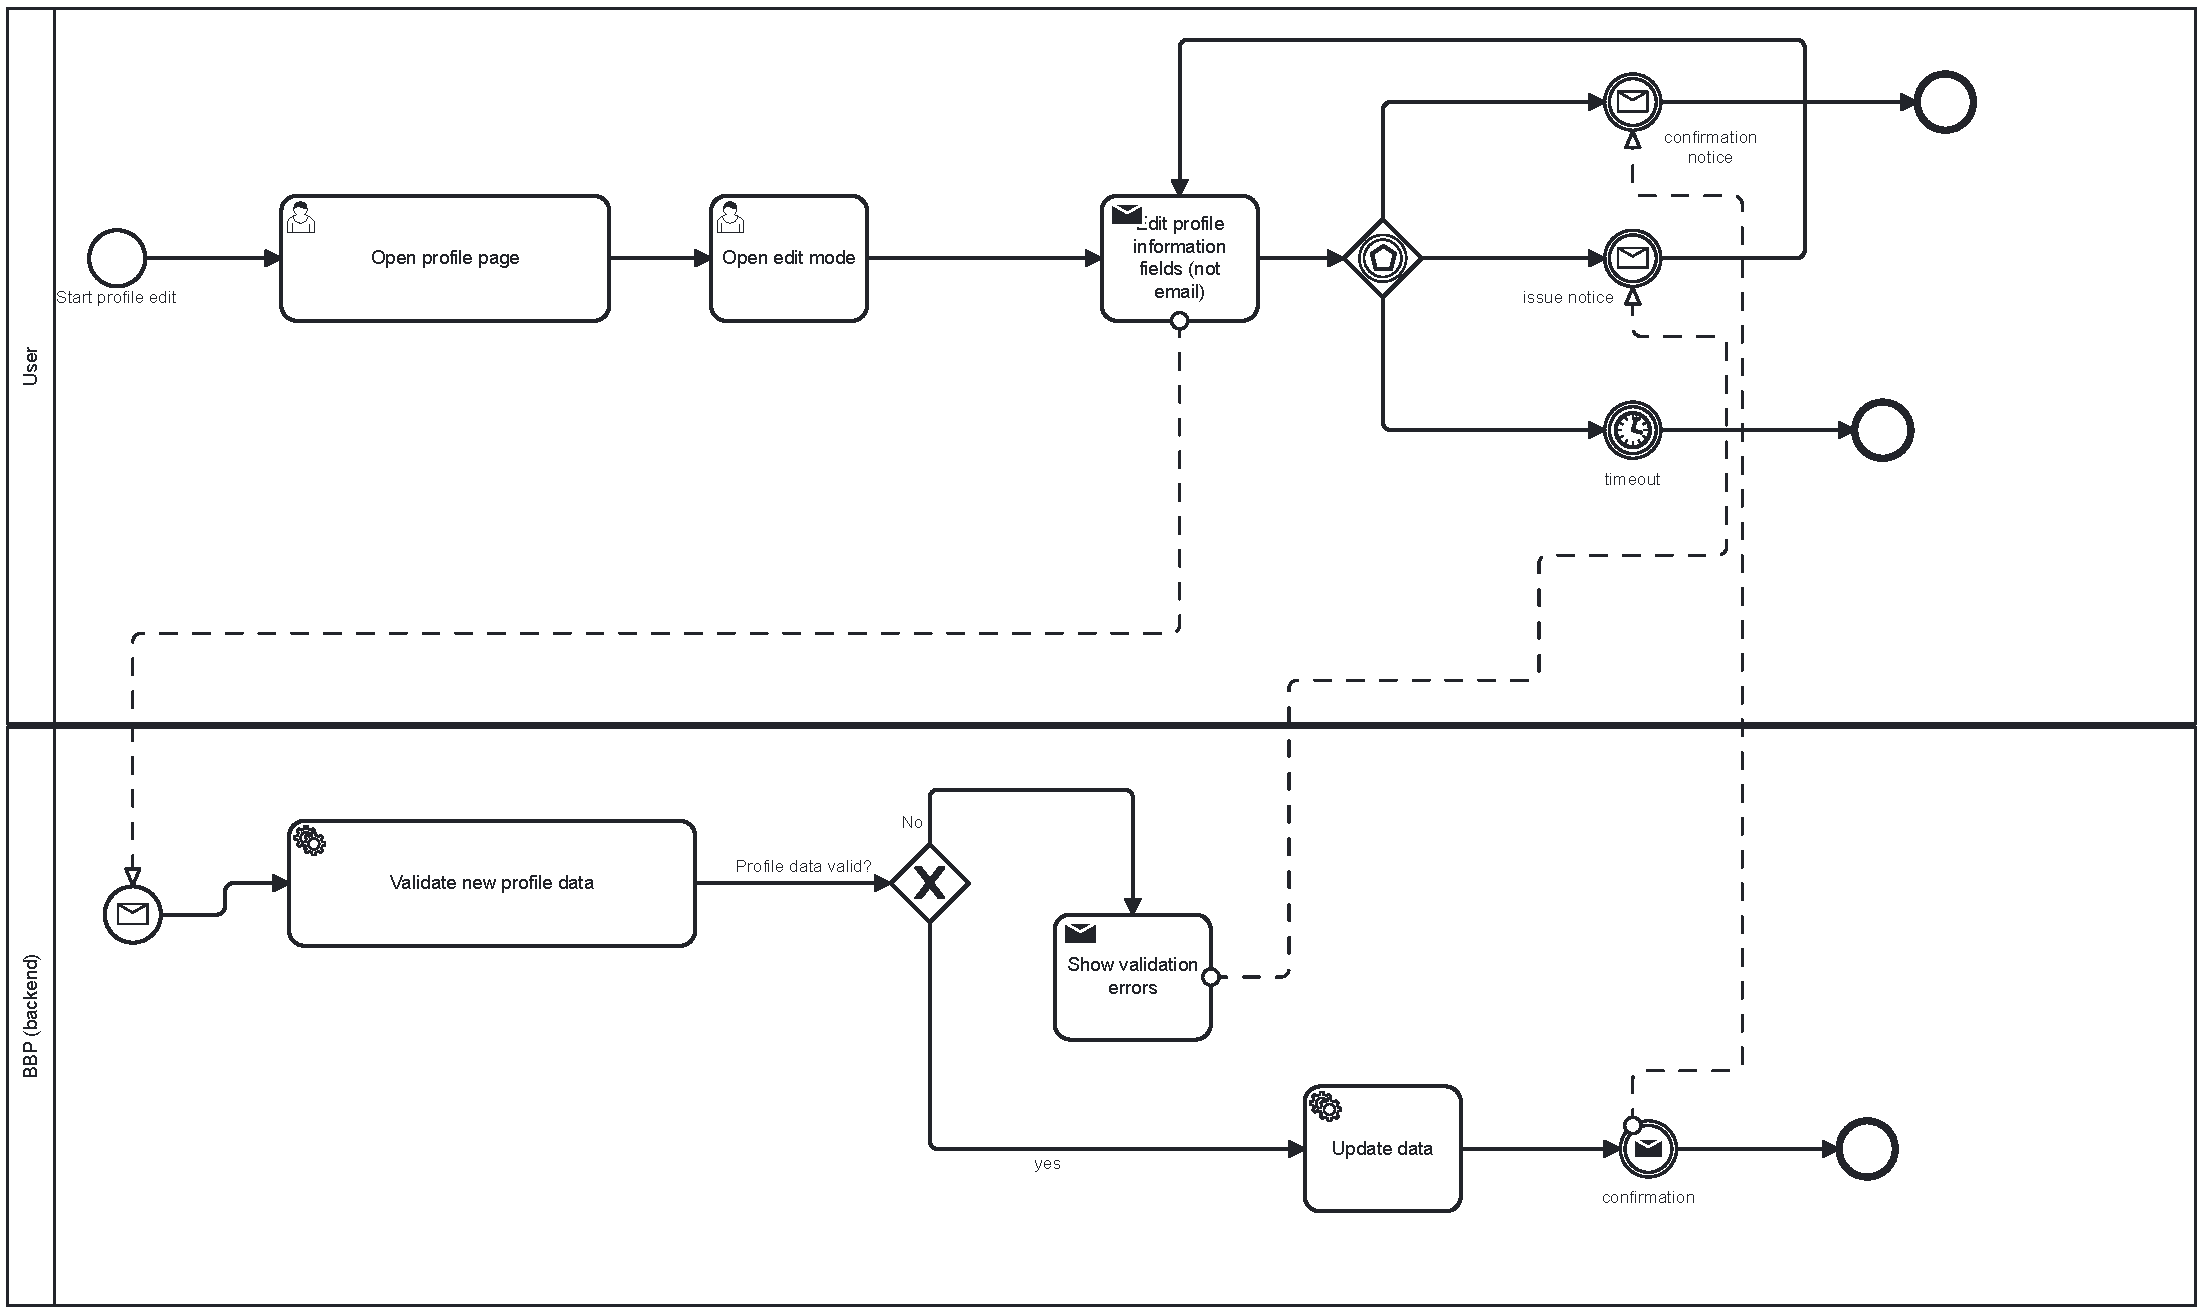
\includegraphics[width=1.0\textwidth]{Images/BPMN/edit-profile.pdf}
                  \caption{Edit profile - Product Function}
                  \label{fig:edit-profile}
            \end{figure}

    
      \item \textbf{Publish Trip}:
Publish Trip is the functionality that allows a registered user to make one of their previously saved cycling trips publicly available, transforming it from a private draft into a shared resource within the Best Bike Paths (BBP) platform. This phase represents a critical transition in the lifecycle of a trip, as additional validation, enrichment, and evaluation processes are triggered exclusively at publication time.

The process starts when the user accesses the saved trips section and selects a specific trip to publish. After confirming the request and providing the required information, the system forwards the publish request to the BBP backend for processing.

Upon receiving the request, the backend initiates a subprocess aimed at improving data quality and consistency. This subprocess searches for other published trips that share one or more streets with the selected trip. If no common streets are found, the trip can be published directly.

If common streets are detected, the backend compares the street-related information contained in the newly published trip with existing data derived from other users’ trips. A decision subprocess evaluates whether discrepancies or differences are present. When differences are identified, the system determines which information should be considered authoritative and updates the status of the affected streets, potentially marking them as problematic. These updates are then published to the shared dataset. This logic adheres to the system's requirement to merge information based on freshness and the number of confirming data points.

During this enrichment and validation phase, the system evaluates the quality of the trip and assigns a trip score. This score is computed exclusively at publication time, as it depends on the comparison with existing trips and on the consistency and reliability of the associated street data. Prior to publication, saved trips do not have an assigned score.

The update process may extend further if additional streets are discovered through other related trips, ensuring that all impacted data remains consistent. If errors occur at any stage of the publishing, comparison, or evaluation process, the procedure is terminated and an error notification is sent to the user.

When the publishing process completes successfully, the user receives a confirmation message. In cases where extended analysis or propagation of updates is required, the user is informed that the trip has been successfully published, but that some updates may take additional time to fully propagate.

            \begin{figure}[H]
                  \centering
                  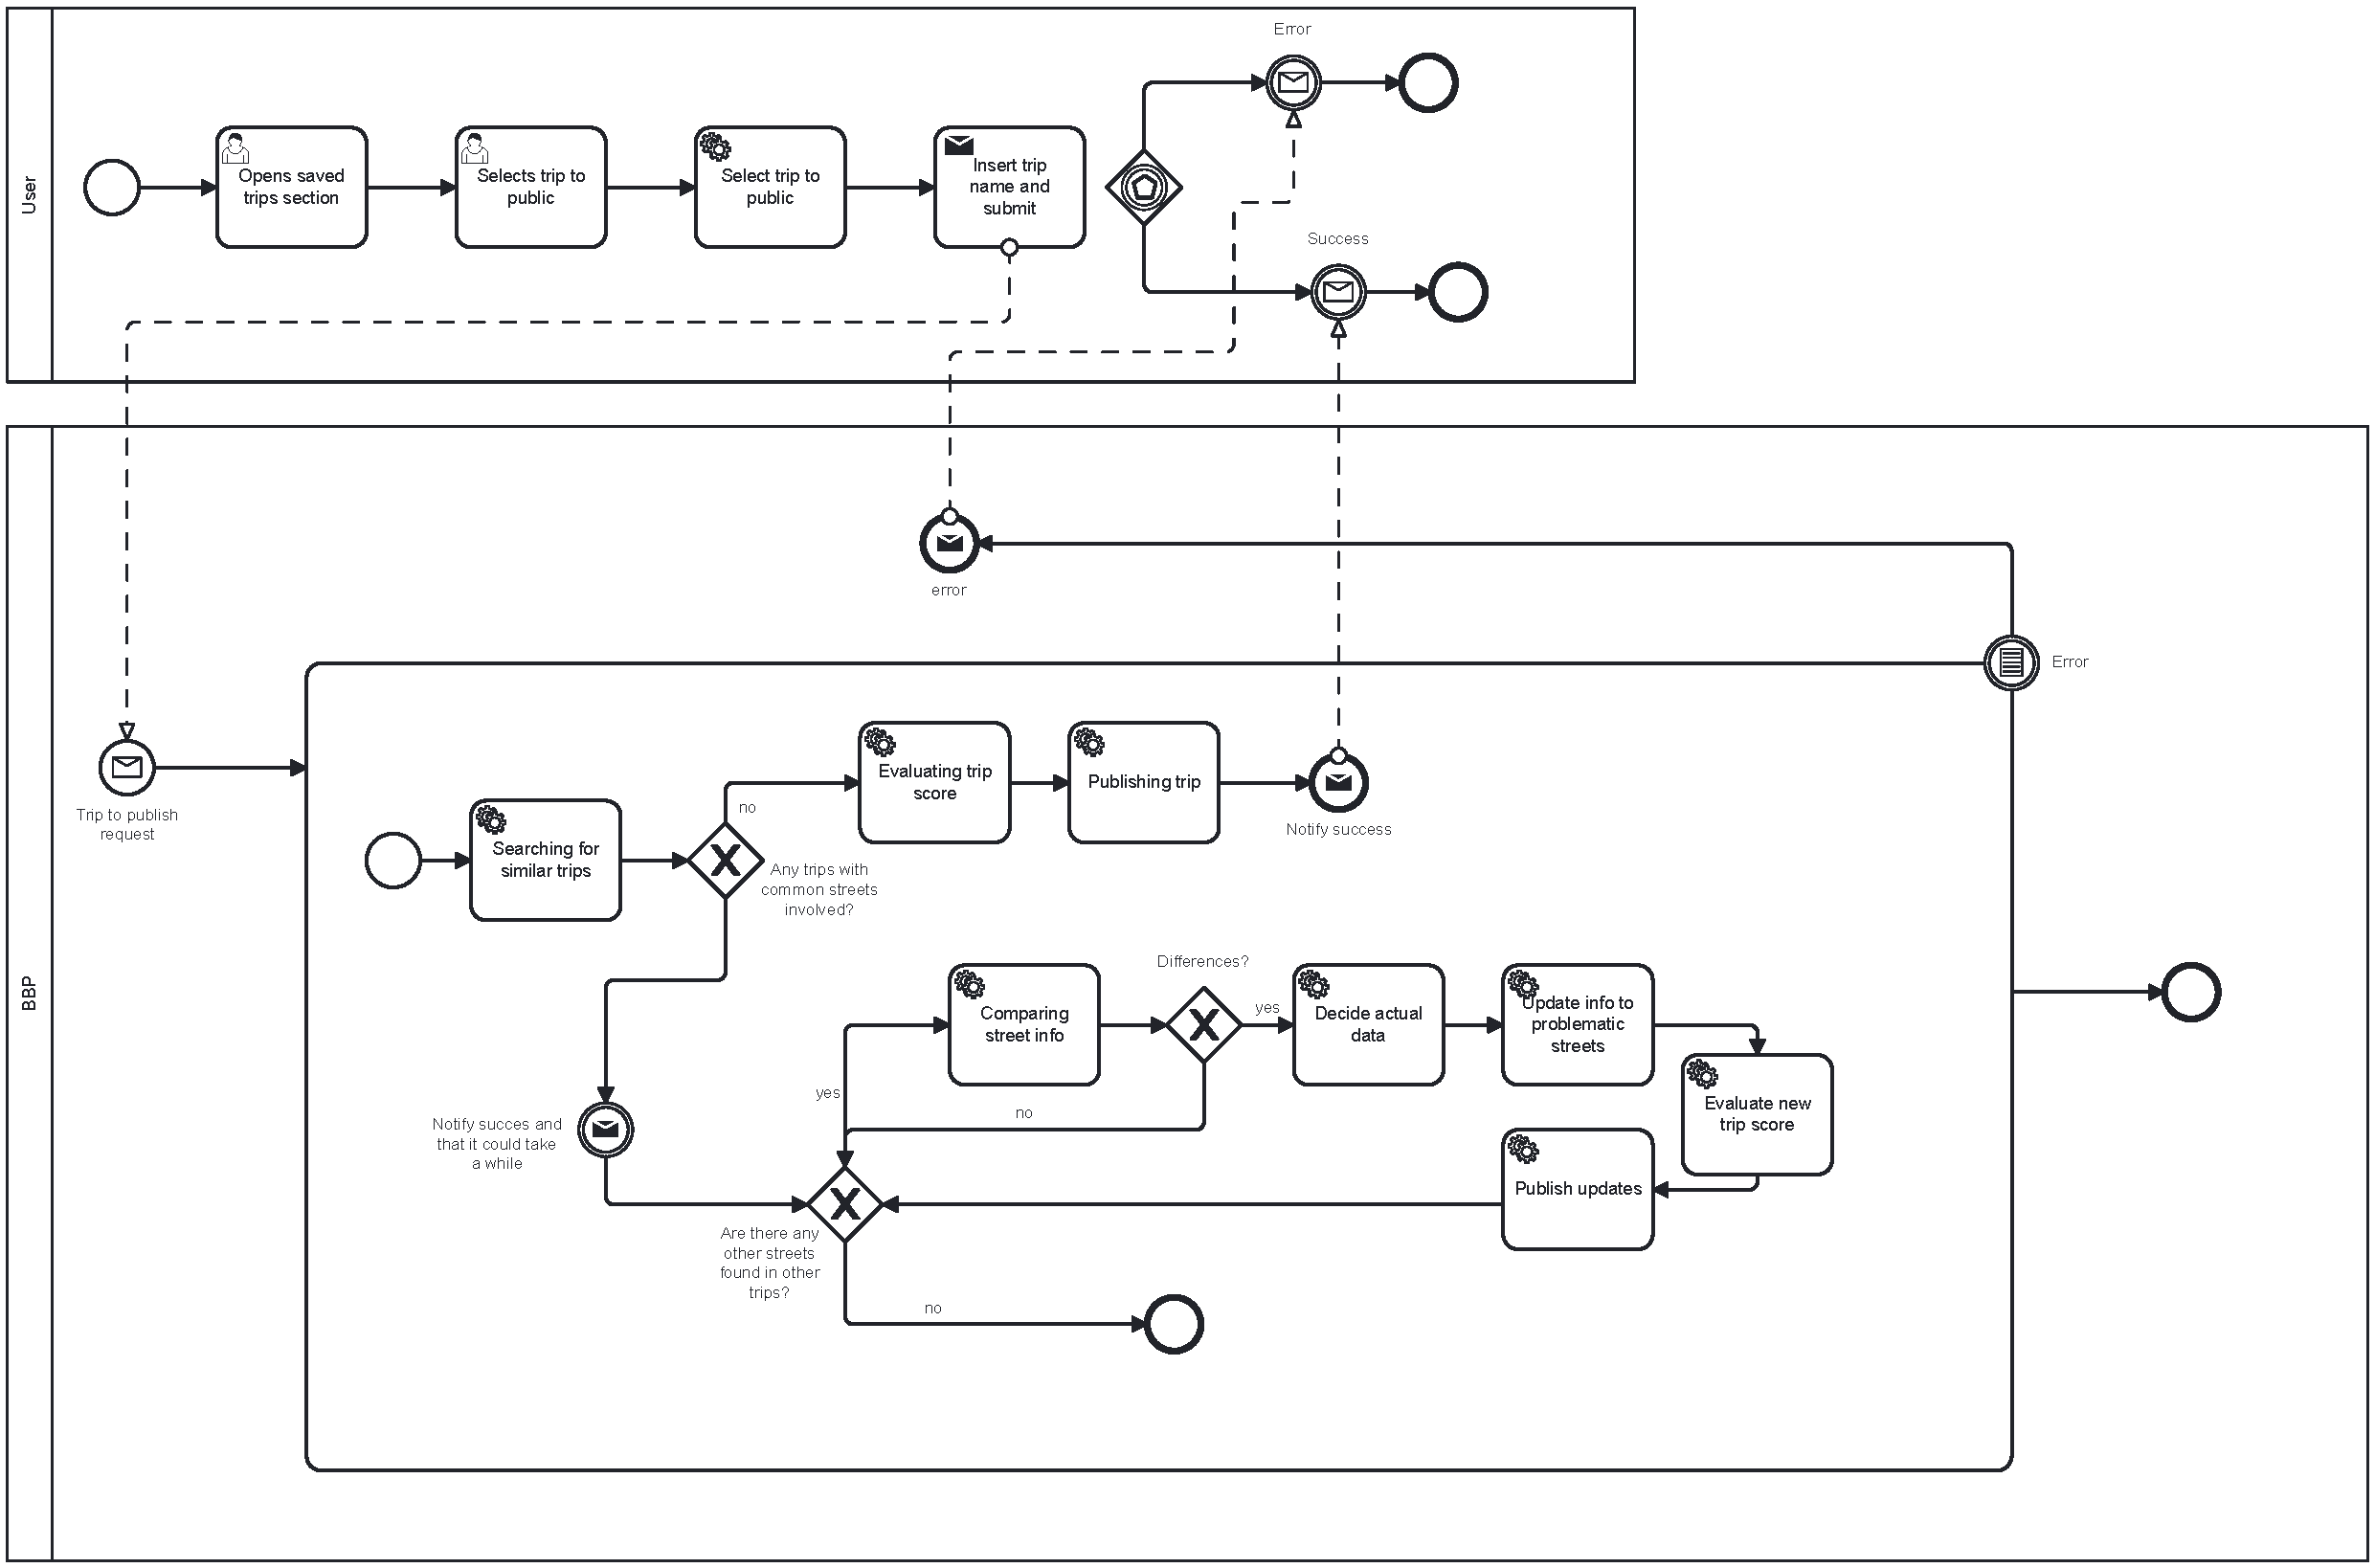
\includegraphics[width=1.0\textwidth]{Images/BPMN/publish_trip.pdf}
                  \caption{Publish Trip - Product Function}
                  \label{fig:publish_trip}
            \end{figure}


\item \textbf{Automatic Trip}:

The Automatic Trip functionality enables the system to record a user's cycling activity in real-time by leveraging the mobile device's onboard sensors, such as the gyroscope, accelerometer, and GPS. The process is initiated when the user opens the recording page and triggers the start command. The system immediately performs a preliminary check to verify if the application has the necessary permissions to access the required sensors. If permissions are missing, the user is prompted to grant them; if the user denies permission, the process cannot proceed.

Once permissions are secured, the system performs a functional check to ensure data is actually being received from the sensors. If no data is detected, the system reports an error and halts the operation. Upon successful validation of sensor availability, the system calibrates the sensors and configures the sampling rate. The recording phase then enters a continuous loop where, for every active sensor within its specific sample interval, the system reads, processes, and aggregates new data. This real-time data is visualized on the user's dashboard until the user explicitly issues a stop recording signal.

After the recording is stopped, the user reviews the trip details and confirms the session. The system attempts to enrich the recorded data with local weather information, if available, before sending the draft data to the BBP backend.

On the backend, the incoming data undergoes a coherence validation process to ensure the integrity of the trip trajectory and sensor metrics. If the data is valid, the trip is saved to the database, and a success notice is sent back to the user. If the data shows inconsistencies, the backend attempts to build suggestions to correct the path before notifying the user. Finally, the client application receives the response and, based on the validity of the street info returned, displays a success visualization to confirm the trip has been stored.

            \begin{figure}[H]
                  \centering
                  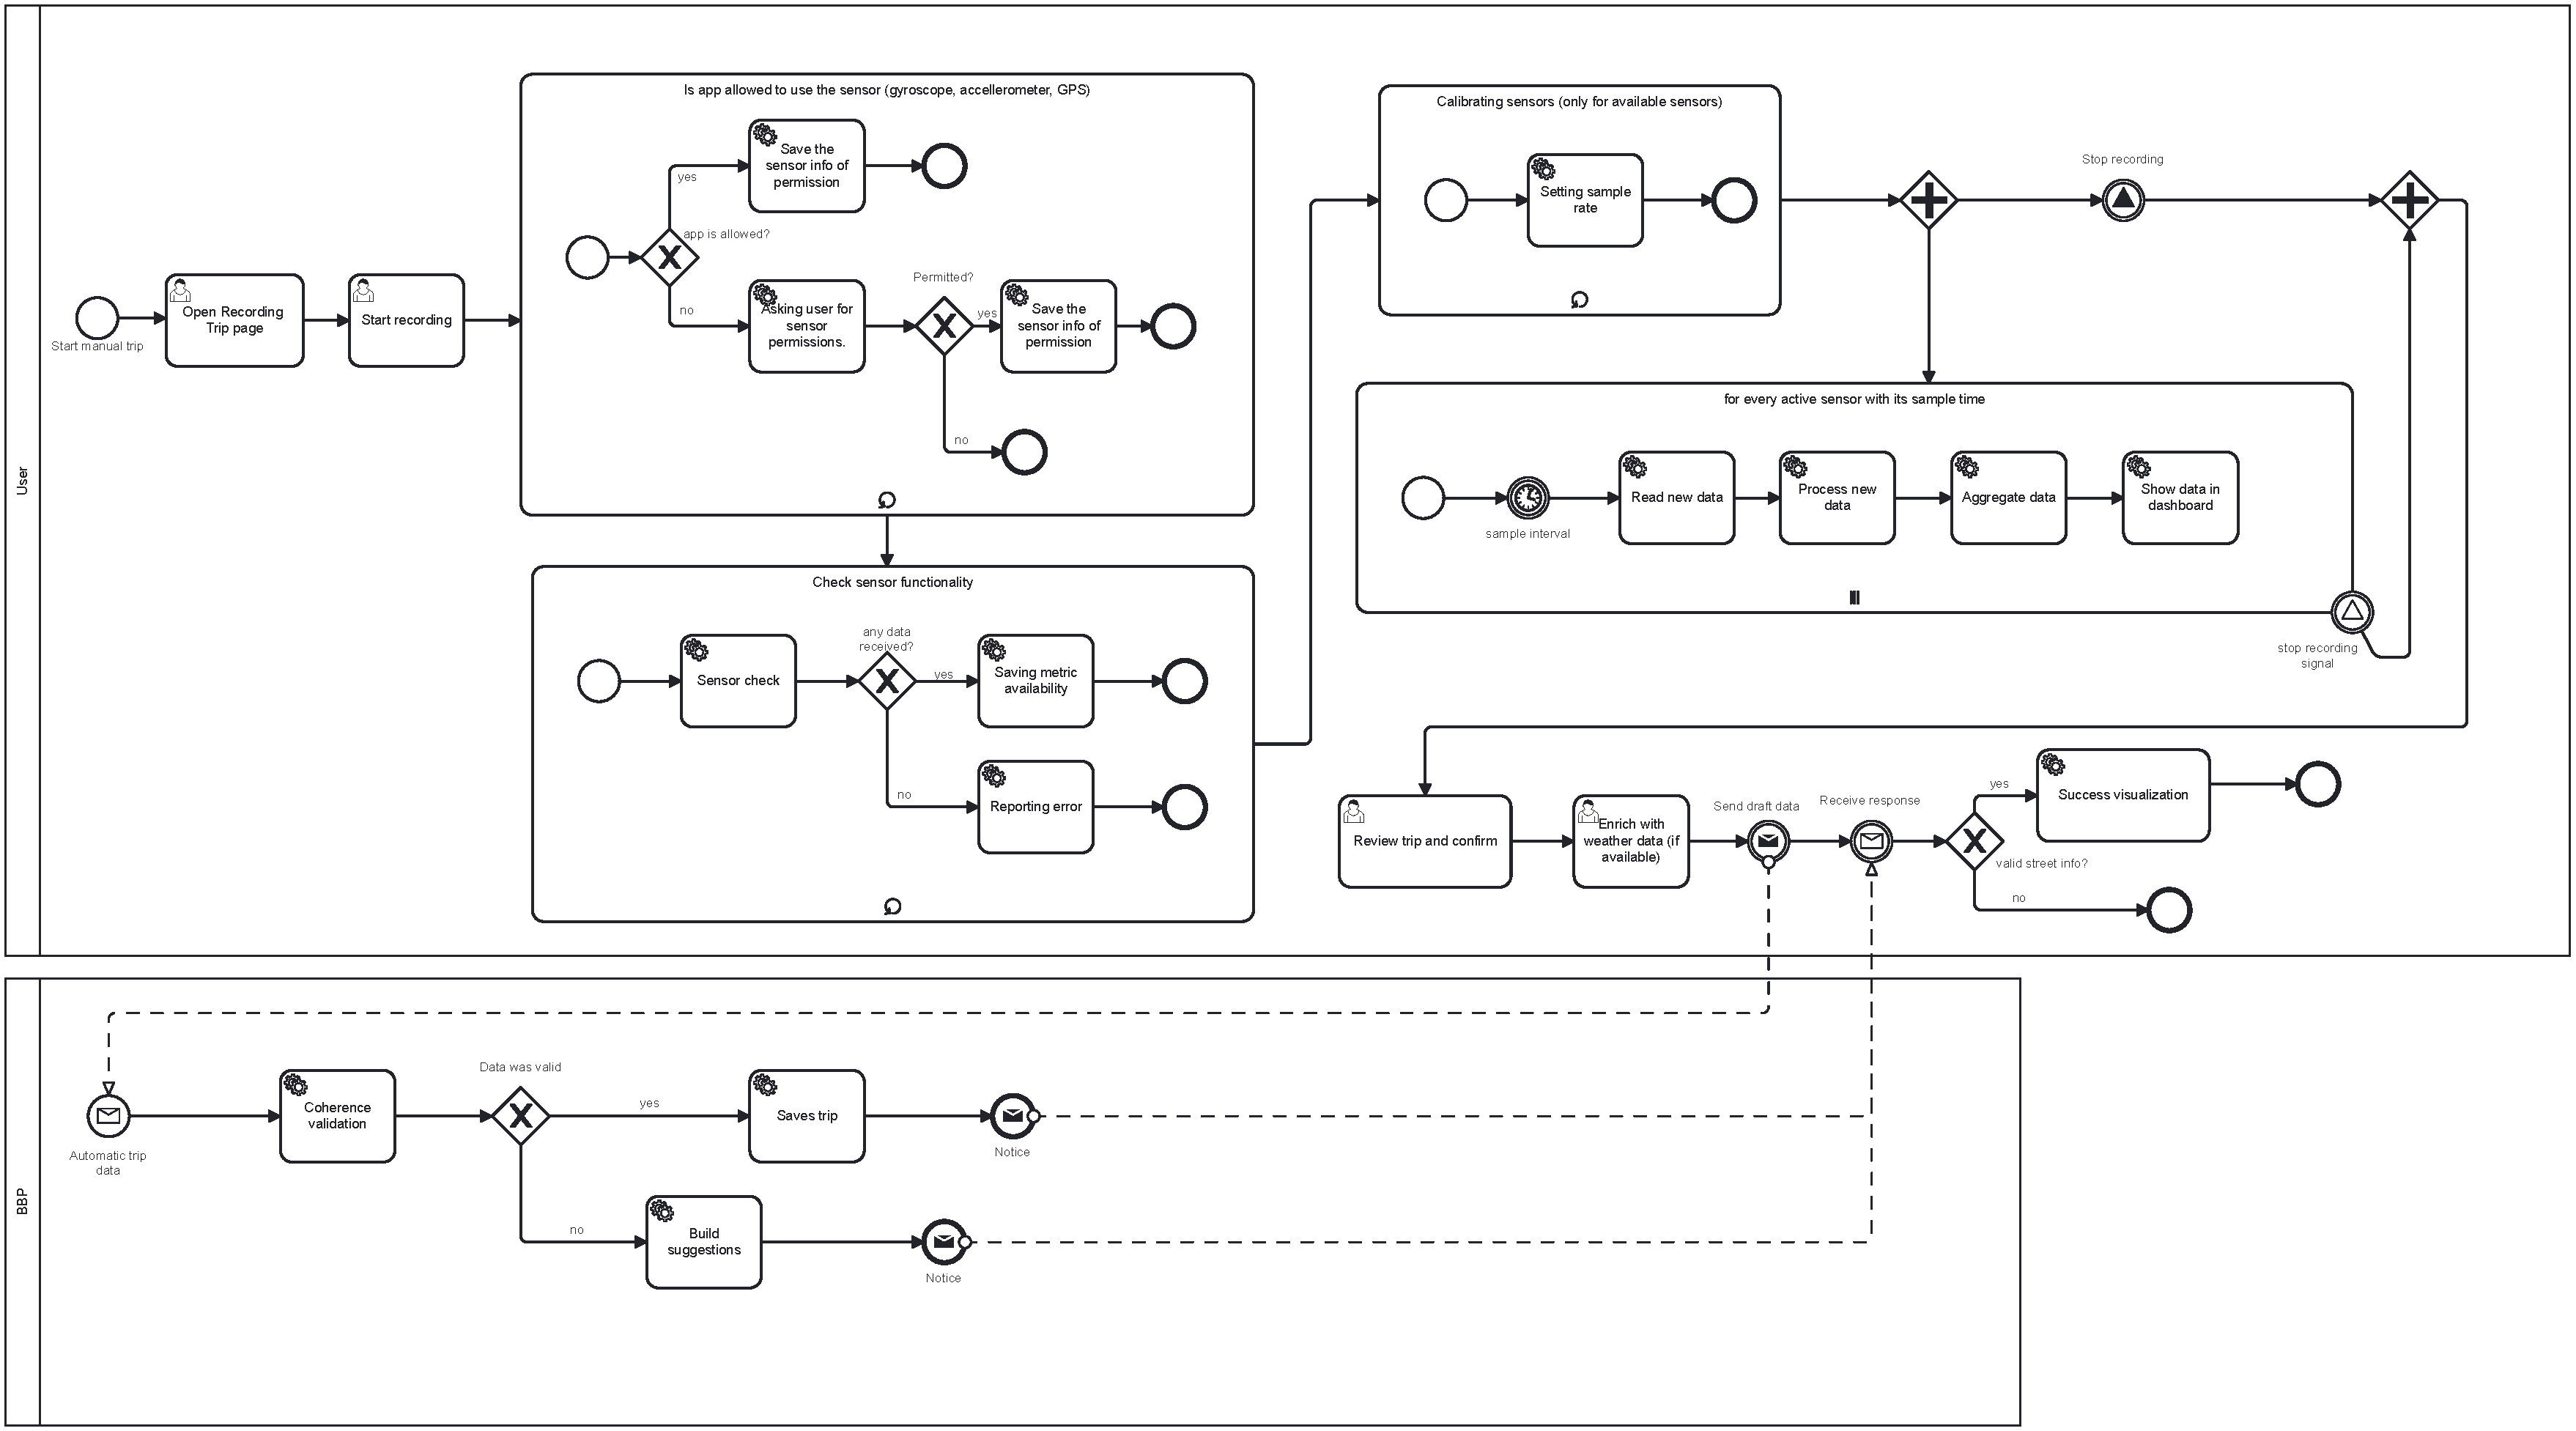
\includegraphics[width=1.0\textwidth]{Images/BPMN/automatic-trip.pdf}
                  \caption{Automatic Trip - Product Function}
                  \label{fig:automatic-trip}
            \end{figure}
\item \textbf{Manual Trip and Edit Trip}:

The Manual Trip and Edit Trip functionalities provide users with the flexibility to document cycling activities retrospectively or modify existing records without relying on real-time sensor recording. This process begins when the user navigates to their personal trips page. At this stage, a decision gateway determines the workflow: the user can either select the option to "create new manual trip" or choose a specific "personal trip to edit".

The core of the trip construction happens through an iterative interaction loop between the user, the BBP backend, and the external OpenStreetMap service. If the user wishes to add a street, they initiate a street search. This request is forwarded by the BBP system to OpenStreetMap, which processes the query and returns the relevant elaboration. The BBP backend then creates an appropriate data object for the street and presents the result to the user. The user then defines the specific path segments and assigns the relevant status to the street. Conversely, if the user needs to correct the route, they can select an already inserted street and delete it.

Once the user determines that the trip composition is complete, they proceed to review the trip details and confirm the submission. Before transmission, the system attempts to enrich the trip information with historical weather data, if available. The draft data is then sent to the backend for final processing.

Upon receiving the finished draft, the BBP system performs a coherence validation to ensure the logical continuity and data integrity of the route. If the data is valid, the system saves the trip and sends a success notice. If the validation fails, the system builds suggestions to rectify the errors and notifies the user, who must then resolve the validity issues before the trip can be successfully stored.

            \begin{figure}[H]
                  \centering
                  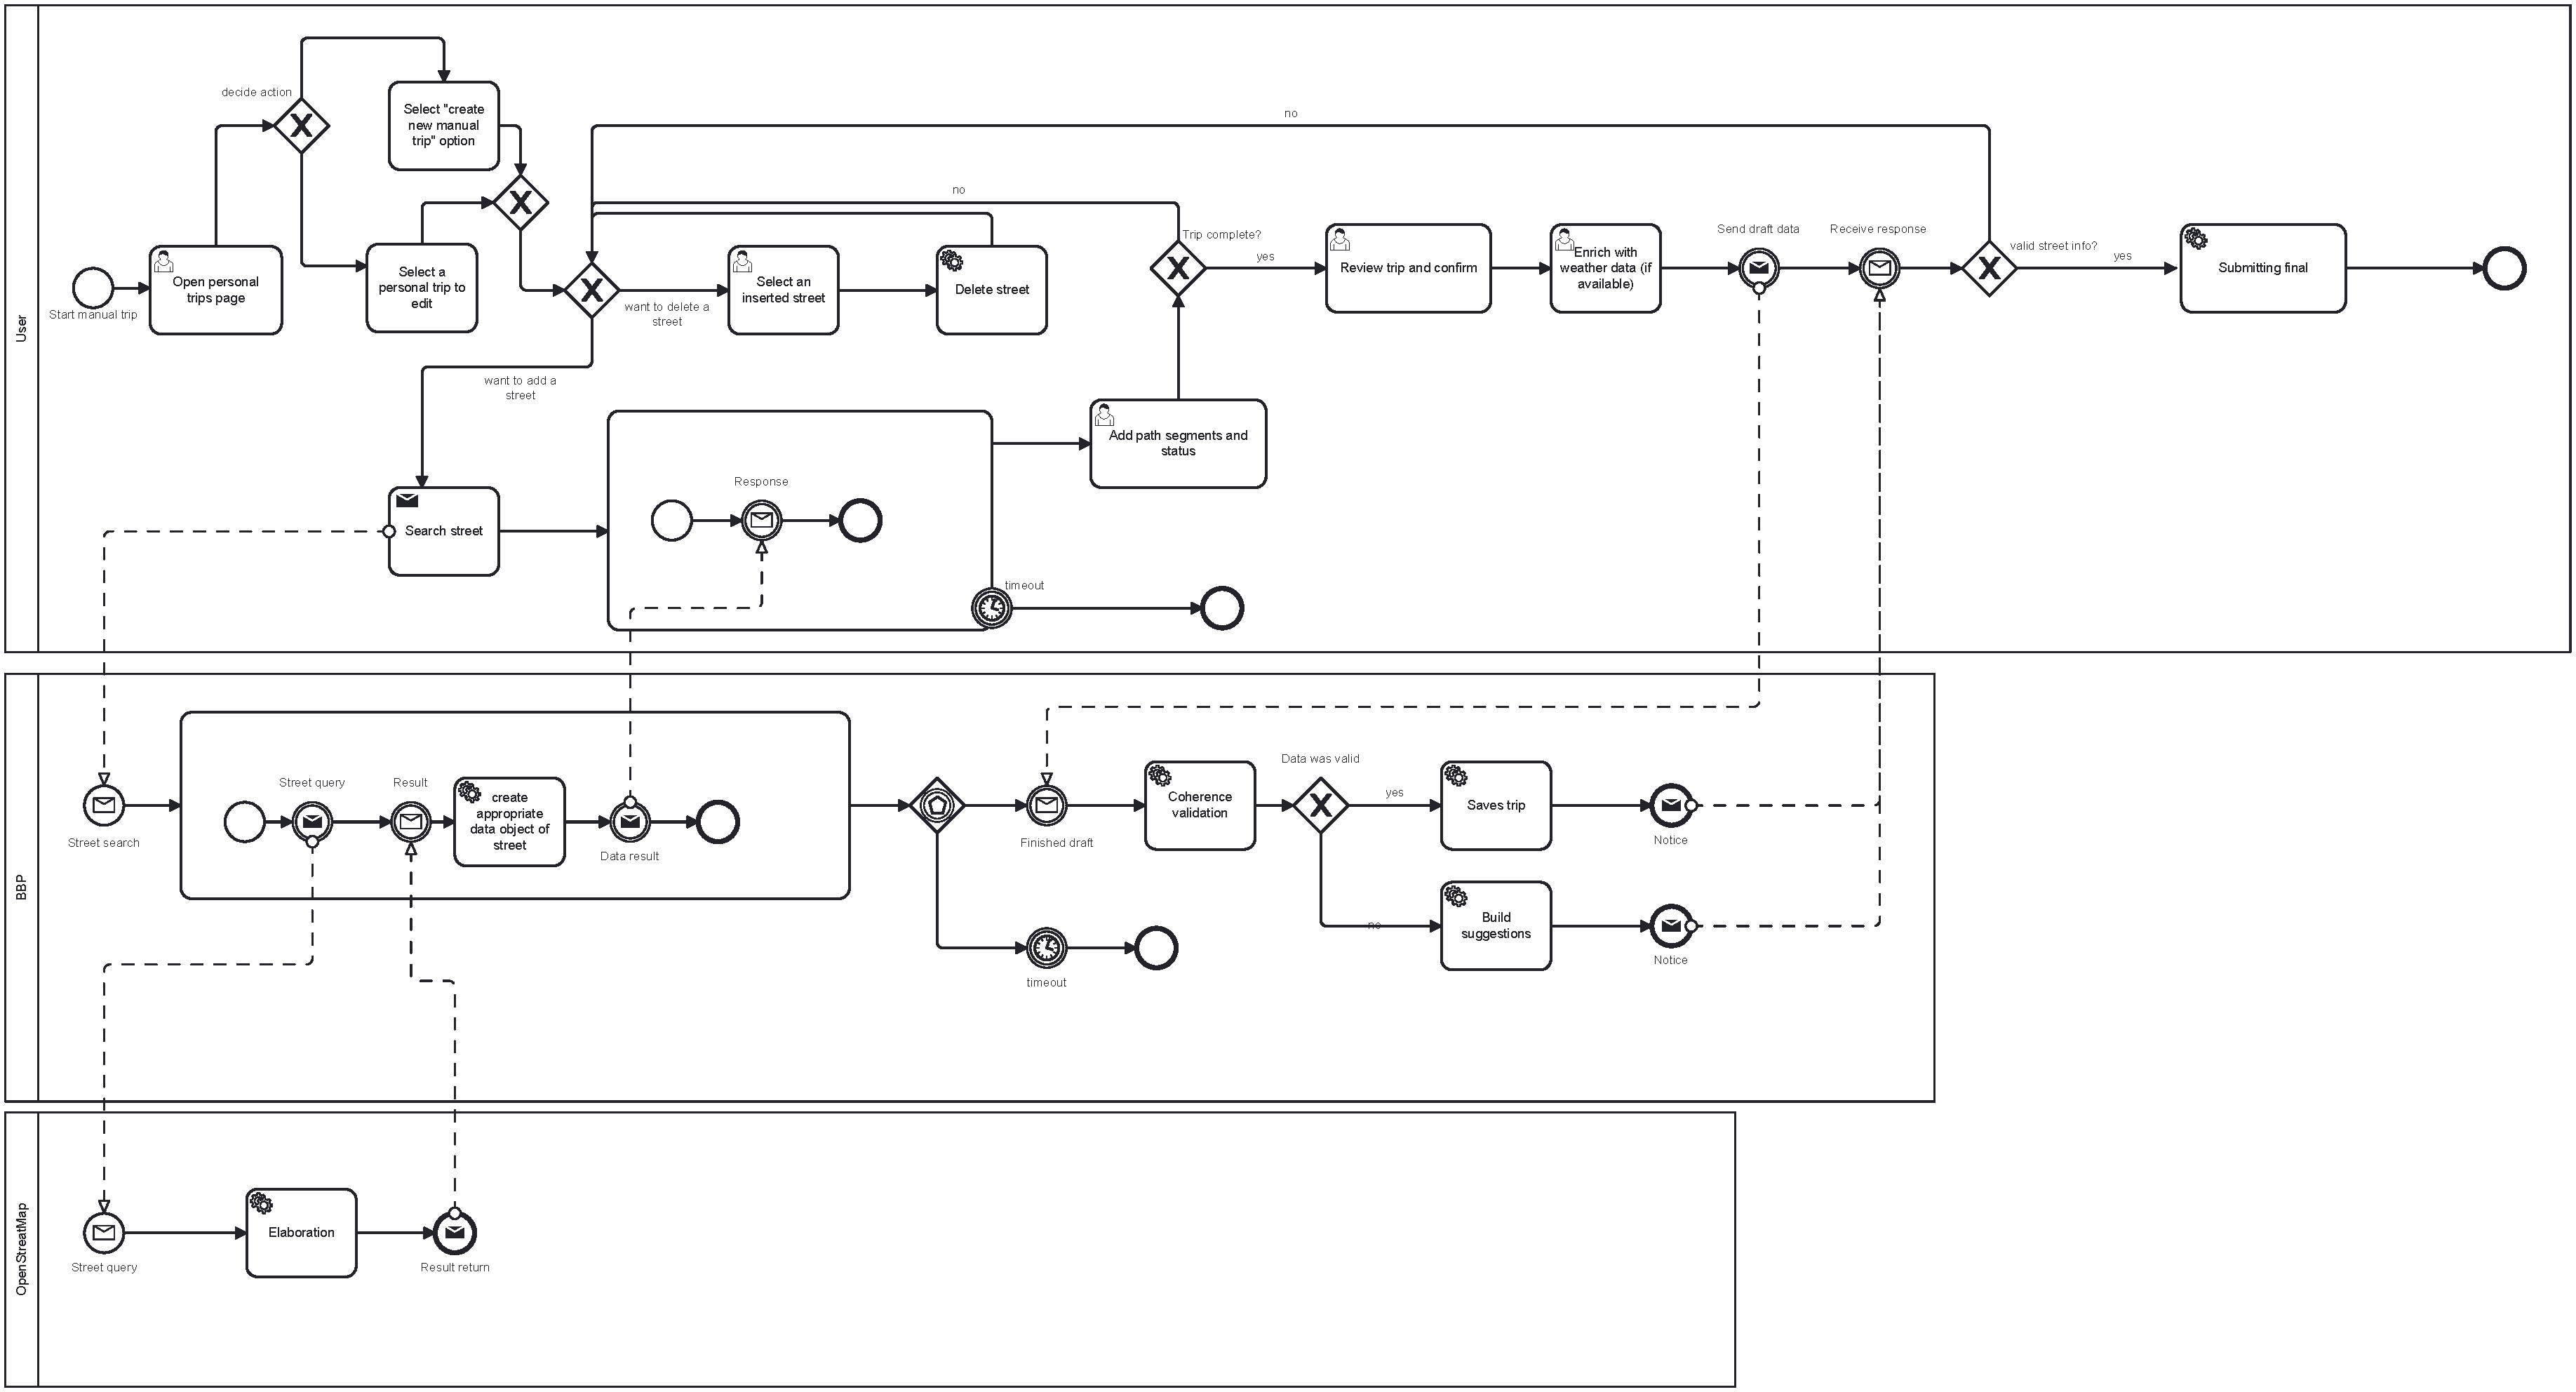
\includegraphics[width=1.0\textwidth]{Images/BPMN/manual-trip_edit-trip.pdf}
                  \caption{Manual Trip and Edit Trip - Product Function}
                  \label{fig:manual-trip_edit-trip}
            \end{figure}


\item \textbf{Search Trip}:

The Search Trip functionality empowers users to discover existing cycling routes within the BBP database based on specific geographical and qualitative criteria. The process begins when the user accesses the search page and defines the parameters for the desired trip. This involves inserting a start position and a final position, choosing the desired distance of the trip, and selecting filter conditions based on the trip score.

Once the criteria are defined and the request is submitted, the BBP backend processes the input by composing and executing a database query. The system then verifies if any data matches the user's search parameters. If no matching trips are found, a negative response is returned to the user. Conversely, if data is available, the backend formats the database results and sends a positive response containing the trip details.

On the client side, the application waits for the server's response, with a timeout mechanism in place to handle potential communication failures. Upon receiving the data, the application formats it for visualization, presenting the results to the user. At this stage, the user is offered the option to sort the results. If the user chooses to sort, they can select a specific sort parameter, prompting the system to re-render the data visualization accordingly. The process concludes when the user is satisfied with the view or chooses not to apply further sorting.

            \begin{figure}[H]
                  \centering
                  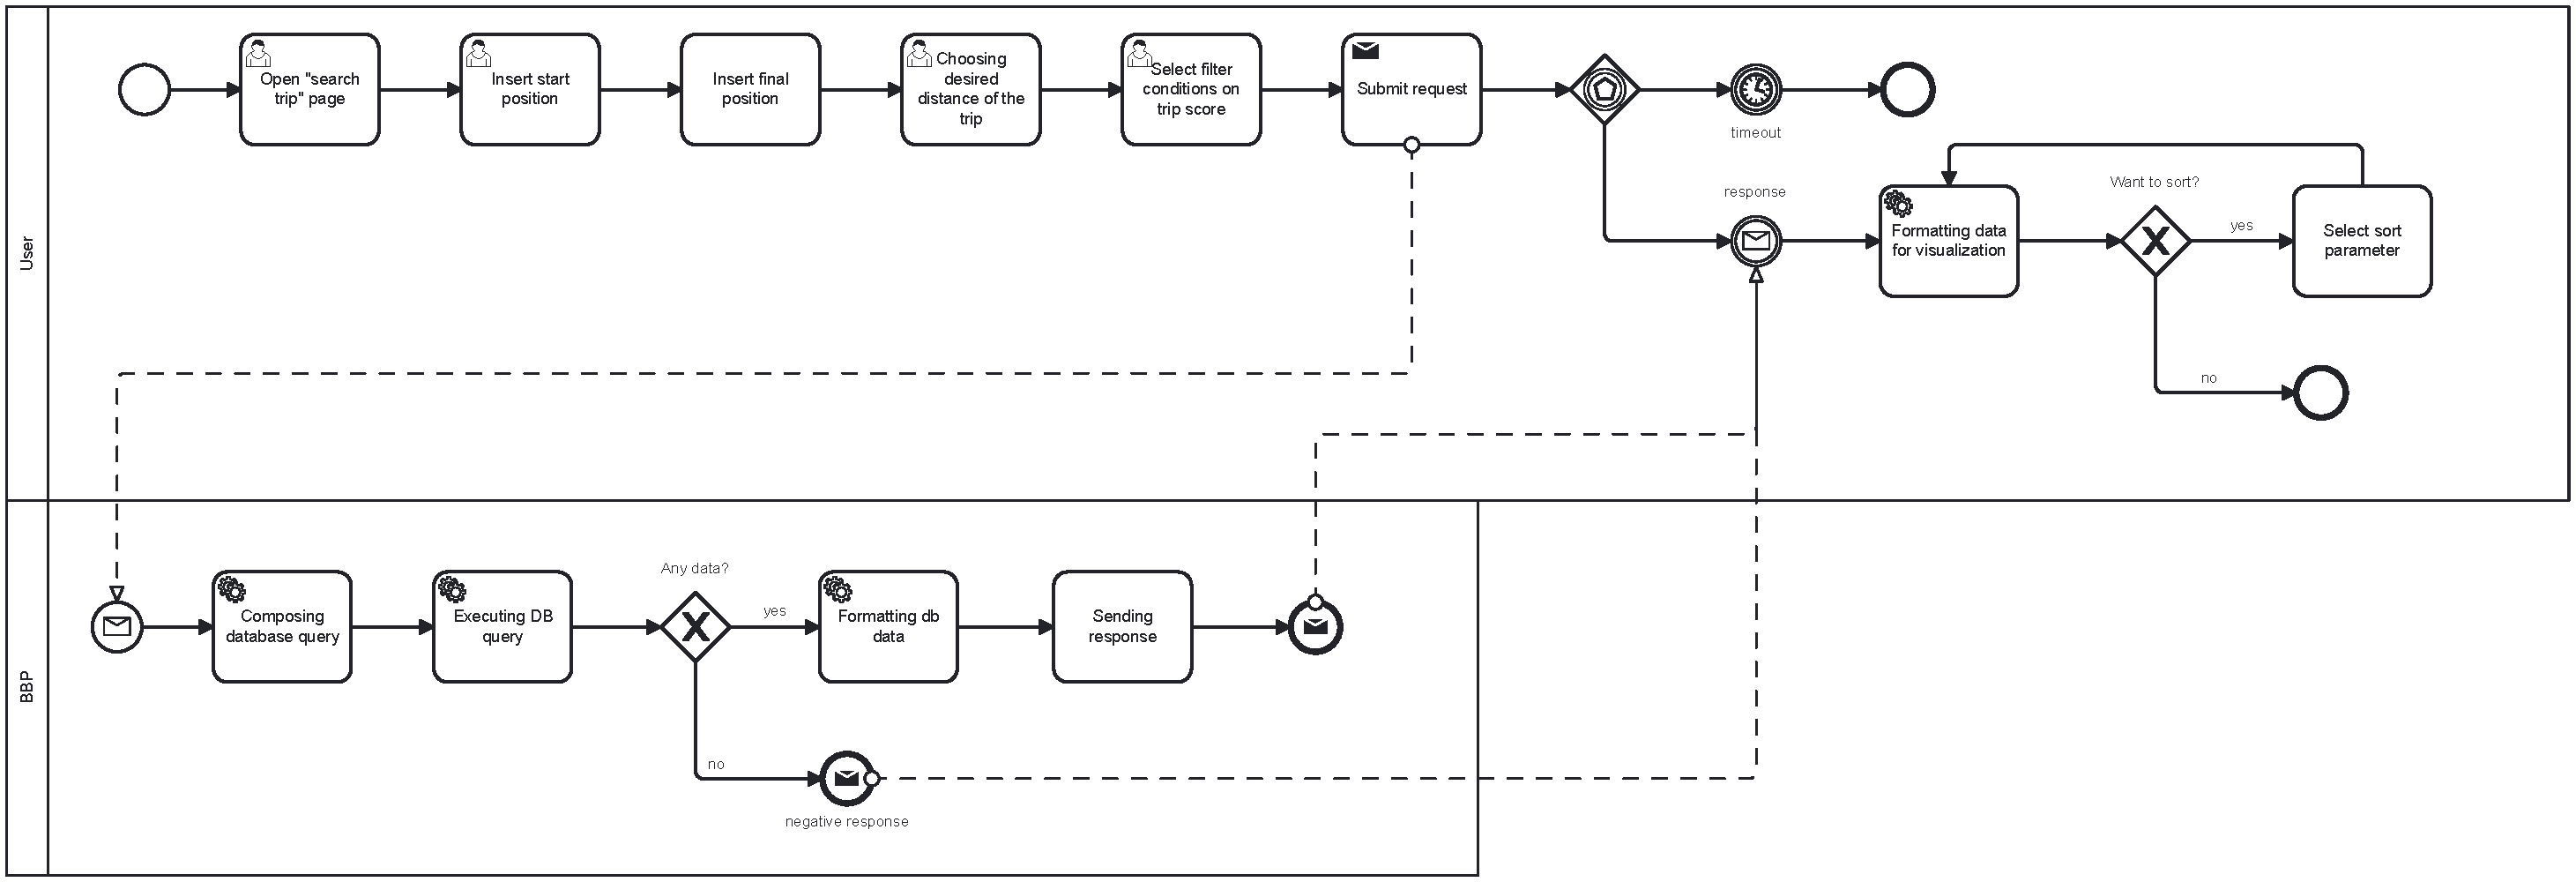
\includegraphics[width=1.0\textwidth]{Images/BPMN/search-trip.pdf}
                  \caption{Search Trip - Product Function}
                  \label{fig:search-trip}
            \end{figure}
\item \textbf{Weather Conditions Retrieval (Subprocess)}:

In several BPMN diagrams related to trip recording and submission, the enrichment of a trip with weather information is represented as a single atomic activity for readability and space constraints. In practice, this activity corresponds to a structured client-side subprocess that interacts with an external weather service.

The subprocess is triggered once a trip recording is completed and before the trip data is sent to the BBP backend. The client application extracts the relevant contextual parameters from the recorded trip, including the geographic position, the date, and the time interval of the activity. These parameters are used to build a request addressed to the external weather service.

The weather service processes the request and attempts to return meteorological information corresponding to the specified location and time, such as temperature, wind conditions, and a qualitative weather status. Upon receiving the response, the client validates its correctness and completeness. If the response is valid, the trip data is enriched with the retrieved weather information and the subprocess terminates successfully.

If the request fails due to a timeout or if the response is invalid or unavailable, the subprocess terminates without enriching the trip. In this case, the absence of weather data does not block the overall trip submission process, which continues with the available information. This design choice ensures robustness against temporary unavailability of external services and maintains a smooth user experience.

Figure~\ref{fig:weather-subprocess} details the internal flow of this subprocess, which is abstracted as a single task in higher-level BPMN diagrams to preserve clarity.
\begin{figure}[H]
    \centering
    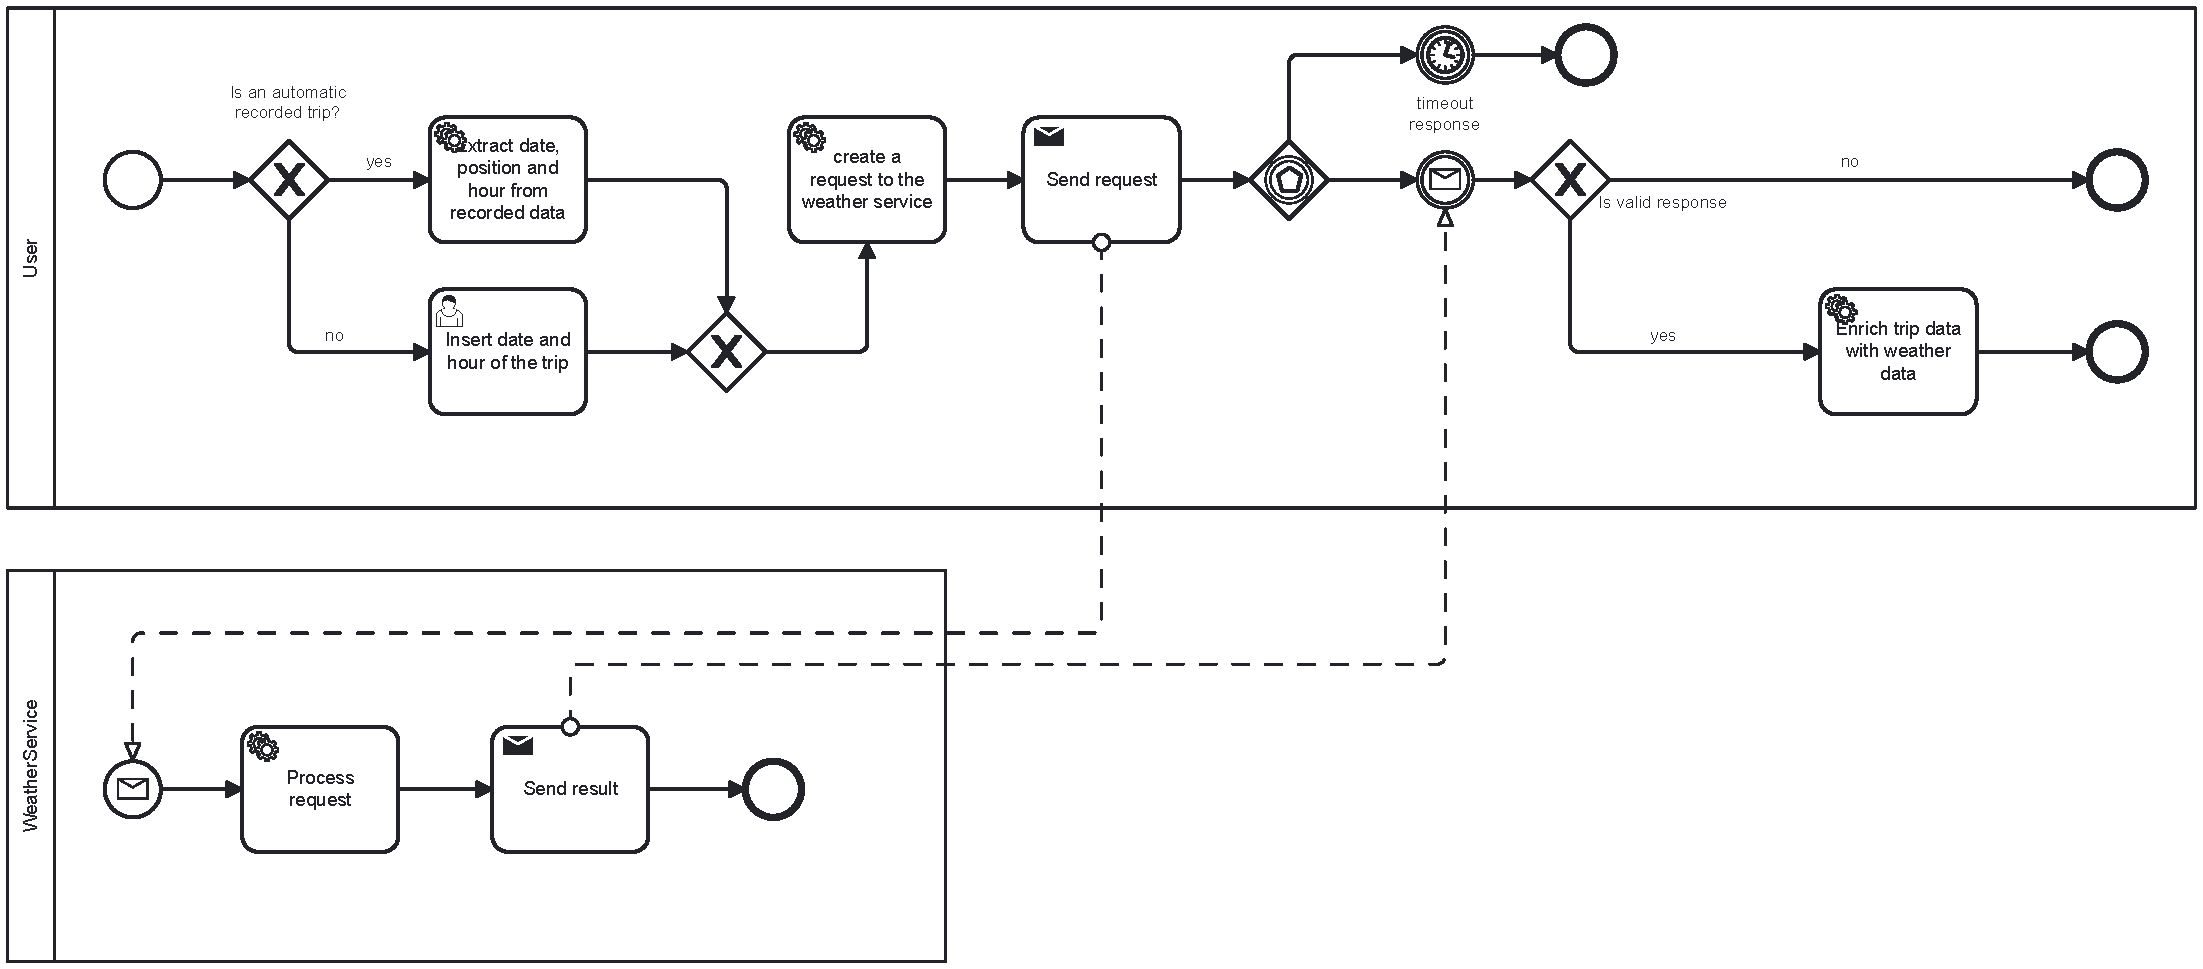
\includegraphics[width=0.9\textwidth]{Images/BPMN/WeatherService.pdf}
    \caption{Weather Conditions Retrieval - Client-side Subprocess}
    \label{fig:weather-subprocess}
\end{figure}
\end{itemize}

\pagebreak

% ============================
% USER CHARACTERISTICS
% ============================

\section{User Characteristics}
\label{sec:user_characteristics}

\par The Best Bike Paths (BBP) system is designed around a single primary actor category: cyclists. These users directly interact with the system by providing information about their trips, obstacles, and the condition of bike paths. Although the platform relies on external map and weather services, these components do not constitute actors, since they do not actively interact with the system as users. Therefore, cyclists represent the only true user-facing category in the domain.

\begin{enumerate}
    \item \textbf{Cyclists (CYs)}: individuals who use the BBP platform while cycling.
    \begin{enumerate}
        \item Cyclists may access the system anonymously or through a registered account.
        \item \textit{Registered cyclists} can record trips, provide feedback on path conditions, report obstacles, and validate automatically detected obstacles.
        \item They may choose whether their reports or feedback become publishable to the community.
        \item \textit{Unregistered cyclists} may only browse aggregated information about paths, obstacles, and cycling conditions, without contributing data.
        \item In both cases, cyclists benefit from enriched information about bike routes, including street conditions and past observations collected from the community.
    \end{enumerate}
\end{enumerate}

\par All additional components (e.g., map providers, weather services, sensors) are external technical dependencies and will be discussed separately in the Design Document.

% ============================
% ASSUMPTIONS, DEPENDENCIES, CONSTRAINTS
% ============================

\section{Assumptions, Dependencies and Constraints}
\label{sec:assumptions_dependencies_and_constraints}

\subsection{Assumptions}
\label{sub:assumptions}

\begin{longtable}{|l|p{0.9\textwidth}|}
\hline
\textbf{Assumption} & \textbf{Description} \\
\hline
A01 & Cyclists use a smartphone capable of running the BBP application and supporting the required sensing features. \\
\hline
A02 & Device location services (GPS) are enabled when using automatic acquisition mode, allowing the system to reconstruct trips reliably. \\
\hline
A03 & Smartphones include functioning motion sensors (such as accelerometers) that can detect vibrations and help identify potential obstacles. \\
\hline
A04 & Cyclists have a stable internet connection during or after their trips to upload data, synchronize reports, and retrieve updated information. \\
\hline
A05 & Users submitting manual path status reports or obstacle reports provide information that reasonably reflects the true conditions of the streets. \\
\hline
A06 & External weather and map providers return accurate, timely, and consistent information used to enrich trip data and support path evaluation. \\
\hline
A07 & The mobile device clock is set correctly, allowing timestamps to be meaningful for trip reconstruction and report creation. \\
\hline
\caption{Domain Assumptions Table}
\label{tab:domain_assumptions}
\end{longtable}

\subsection{Dependencies}
\label{sub:dependencies}

\begin{longtable}{|l|p{0.9\textwidth}|}
\hline
\textbf{Dependency} & \textbf{Description} \\
\hline
D01 & The system depends on external map services to retrieve geographic data, validate street names, compute paths, and represent routes. \\
\hline
D02 & The system depends on external weather providers to retrieve real-time or historical weather conditions associated with trips. \\
\hline
D03 & The mobile operating system must grant the application access to device sensors such as GPS, accelerometers, and motion detectors. \\
\hline
D04 & The application requires stable internet connectivity for synchronizing trips, uploading reports, downloading path conditions, and retrieving external data. \\
\hline
D05 & Mobile platform APIs must function correctly to access background location updates during trips. \\
\hline
\caption{Domain Dependencies Table}
\label{tab:domain_dependencies}
\end{longtable}

\subsection{Constraints}
\label{sub:constraints}

\begin{longtable}{|l|p{0.9\textwidth}|}
\hline
\textbf{Constraint} & \textbf{Description} \\
\hline
C01 & The system must comply with data protection and privacy regulations concerning the collection, processing, and storage of cyclists' location data. \\
\hline
C02 & BBP must operate on mobile devices with heterogeneous hardware capabilities, meaning data quality may vary across devices. \\
\hline
C03 & The system is constrained by sensor precision: inaccurate GPS, unstable accelerometer readings, or motion sensor noise may impact trip reconstruction and obstacle detection. \\
\hline
C04 & Only publishable and validated data (e.g., confirmed obstacles and user-approved reports) can be displayed to the community. \\
\hline
C05 & The platform should remain functional even with intermittent connectivity, but certain operations (such as uploading data or fetching updated path statuses) are limited without internet access. \\
\hline
C06 & Device battery consumption must be considered, as continuous GPS and sensor usage can reduce battery life during long trips. \\
\hline
\caption{Domain Constraints Table}
\label{tab:domain_constraints}
\end{longtable}